\documentclass[11pt]{article}
\usepackage[T1]{fontenc}
\usepackage{lmodern}
\usepackage[margin=2.5cm]{geometry}
\usepackage{amsmath,amssymb}
\usepackage{graphicx}
\usepackage{booktabs}
\usepackage{setspace}
\usepackage[numbers,sort&compress]{natbib}
\usepackage[hidelinks]{hyperref}
\usepackage{xurl}
\usepackage{lineno}
\setstretch{1.4}
\emergencystretch=2em
% generated by code/make_macros.py -- do not edit
\makeatletter
\expandafter\def\csname res@alertsActualMax\endcsname{12.3}
\expandafter\def\csname res@alertsActualMin\endcsname{7.1}
\expandafter\def\csname res@alertsArone\endcsname{9.7}
\expandafter\def\csname res@alertsBias\endcsname{10.4}
\expandafter\def\csname res@alertsExactMax\endcsname{13.8}
\expandafter\def\csname res@alertsExactMin\endcsname{13.8}
\expandafter\def\csname res@alertsIso\endcsname{10.2}
\expandafter\def\csname res@alertsIsobc\endcsname{10.2}
\expandafter\def\csname res@alertsMax\endcsname{12.9}
\expandafter\def\csname res@alertsMeightMax\endcsname{16.4}
\expandafter\def\csname res@alertsMeightMin\endcsname{13.7}
\expandafter\def\csname res@alertsMin\endcsname{9.7}
\expandafter\def\csname res@alertsMix\endcsname{10.7}
\expandafter\def\csname res@alertsMl\endcsname{10.5}
\expandafter\def\csname res@alertsMthreeMax\endcsname{8.7}
\expandafter\def\csname res@alertsMthreeMin\endcsname{7.0}
\expandafter\def\csname res@alertsNoise\endcsname{9.9}
\expandafter\def\csname res@alertsPers\endcsname{10.3}
\expandafter\def\csname res@alertsShrink\endcsname{12.9}
\expandafter\def\csname res@alertsUnder\endcsname{10.2}
\expandafter\def\csname res@alertsWeek\endcsname{11.2}
\expandafter\def\csname res@alertsWfiveMax\endcsname{12.9}
\expandafter\def\csname res@alertsWfiveMin\endcsname{9.7}
\expandafter\def\csname res@alertsWoneMax\endcsname{12.9}
\expandafter\def\csname res@alertsWoneMin\endcsname{9.7}
\expandafter\def\csname res@budgetErcot\endcsname{20}
\expandafter\def\csname res@budgetIsone\endcsname{5}
\expandafter\def\csname res@budgetMean\endcsname{13.8}
\expandafter\def\csname res@budgetNyiso\endcsname{5}
\expandafter\def\csname res@budgetPjm\endcsname{25}
\expandafter\def\csname res@capArone\endcsname{66}
\expandafter\def\csname res@capAroneActual\endcsname{61}
\expandafter\def\csname res@capAroneErcot\endcsname{44}
\expandafter\def\csname res@capAroneExact\endcsname{79}
\expandafter\def\csname res@capAroneIsone\endcsname{89}
\expandafter\def\csname res@capAroneMeight\endcsname{70}
\expandafter\def\csname res@capAroneMthree\endcsname{56}
\expandafter\def\csname res@capAroneNyiso\endcsname{78}
\expandafter\def\csname res@capAronePjm\endcsname{53}
\expandafter\def\csname res@capAroneWfive\endcsname{75}
\expandafter\def\csname res@capAroneWone\endcsname{35}
\expandafter\def\csname res@capBias\endcsname{82}
\expandafter\def\csname res@capBiasActual\endcsname{86}
\expandafter\def\csname res@capBiasErcot\endcsname{50}
\expandafter\def\csname res@capBiasExact\endcsname{100}
\expandafter\def\csname res@capBiasIsone\endcsname{100}
\expandafter\def\csname res@capBiasMeight\endcsname{85}
\expandafter\def\csname res@capBiasMthree\endcsname{72}
\expandafter\def\csname res@capBiasNyiso\endcsname{100}
\expandafter\def\csname res@capBiasPjm\endcsname{78}
\expandafter\def\csname res@capBiasWfive\endcsname{82}
\expandafter\def\csname res@capBiasWone\endcsname{82}
\expandafter\def\csname res@capIso\endcsname{72}
\expandafter\def\csname res@capIsoActual\endcsname{73}
\expandafter\def\csname res@capIsoErcot\endcsname{47}
\expandafter\def\csname res@capIsoExact\endcsname{85}
\expandafter\def\csname res@capIsoIsone\endcsname{89}
\expandafter\def\csname res@capIsoMeight\endcsname{75}
\expandafter\def\csname res@capIsoMthree\endcsname{65}
\expandafter\def\csname res@capIsoNyiso\endcsname{100}
\expandafter\def\csname res@capIsoPjm\endcsname{51}
\expandafter\def\csname res@capIsoWfive\endcsname{77}
\expandafter\def\csname res@capIsoWone\endcsname{50}
\expandafter\def\csname res@capIsobc\endcsname{77}
\expandafter\def\csname res@capIsobcActual\endcsname{79}
\expandafter\def\csname res@capIsobcErcot\endcsname{50}
\expandafter\def\csname res@capIsobcExact\endcsname{90}
\expandafter\def\csname res@capIsobcIsone\endcsname{89}
\expandafter\def\csname res@capIsobcMeight\endcsname{81}
\expandafter\def\csname res@capIsobcMthree\endcsname{71}
\expandafter\def\csname res@capIsobcNyiso\endcsname{100}
\expandafter\def\csname res@capIsobcPjm\endcsname{69}
\expandafter\def\csname res@capIsobcWfive\endcsname{77}
\expandafter\def\csname res@capIsobcWone\endcsname{52}
\expandafter\def\csname res@capMix\endcsname{69}
\expandafter\def\csname res@capMixErcot\endcsname{31}
\expandafter\def\csname res@capMixIsone\endcsname{89}
\expandafter\def\csname res@capMixNyiso\endcsname{89}
\expandafter\def\csname res@capMixPjm\endcsname{69}
\expandafter\def\csname res@capMl\endcsname{41}
\expandafter\def\csname res@capMlActual\endcsname{15}
\expandafter\def\csname res@capMlErcot\endcsname{17}
\expandafter\def\csname res@capMlExact\endcsname{46}
\expandafter\def\csname res@capMlIsone\endcsname{67}
\expandafter\def\csname res@capMlMeight\endcsname{47}
\expandafter\def\csname res@capMlMthree\endcsname{33}
\expandafter\def\csname res@capMlNyiso\endcsname{33}
\expandafter\def\csname res@capMlPjm\endcsname{49}
\expandafter\def\csname res@capMlWfive\endcsname{52}
\expandafter\def\csname res@capMlWone\endcsname{19}
\expandafter\def\csname res@capNoise\endcsname{61}
\expandafter\def\csname res@capNoiseActual\endcsname{68}
\expandafter\def\csname res@capNoiseErcot\endcsname{39}
\expandafter\def\csname res@capNoiseExact\endcsname{75}
\expandafter\def\csname res@capNoiseIsone\endcsname{78}
\expandafter\def\csname res@capNoiseMeight\endcsname{66}
\expandafter\def\csname res@capNoiseMthree\endcsname{58}
\expandafter\def\csname res@capNoiseNyiso\endcsname{89}
\expandafter\def\csname res@capNoisePjm\endcsname{38}
\expandafter\def\csname res@capNoiseWfive\endcsname{71}
\expandafter\def\csname res@capNoiseWone\endcsname{31}
\expandafter\def\csname res@capPers\endcsname{53}
\expandafter\def\csname res@capPersErcot\endcsname{33}
\expandafter\def\csname res@capPersIsone\endcsname{67}
\expandafter\def\csname res@capPersNyiso\endcsname{67}
\expandafter\def\csname res@capPersPjm\endcsname{47}
\expandafter\def\csname res@capShrink\endcsname{84}
\expandafter\def\csname res@capShrinkActual\endcsname{50}
\expandafter\def\csname res@capShrinkErcot\endcsname{47}
\expandafter\def\csname res@capShrinkExact\endcsname{97}
\expandafter\def\csname res@capShrinkIsone\endcsname{100}
\expandafter\def\csname res@capShrinkMeight\endcsname{87}
\expandafter\def\csname res@capShrinkMthree\endcsname{76}
\expandafter\def\csname res@capShrinkNyiso\endcsname{100}
\expandafter\def\csname res@capShrinkPjm\endcsname{89}
\expandafter\def\csname res@capShrinkWfive\endcsname{85}
\expandafter\def\csname res@capShrinkWone\endcsname{78}
\expandafter\def\csname res@capUnder\endcsname{83}
\expandafter\def\csname res@capUnderActual\endcsname{76}
\expandafter\def\csname res@capUnderErcot\endcsname{53}
\expandafter\def\csname res@capUnderExact\endcsname{100}
\expandafter\def\csname res@capUnderIsone\endcsname{100}
\expandafter\def\csname res@capUnderMeight\endcsname{85}
\expandafter\def\csname res@capUnderMthree\endcsname{75}
\expandafter\def\csname res@capUnderNyiso\endcsname{100}
\expandafter\def\csname res@capUnderPjm\endcsname{78}
\expandafter\def\csname res@capUnderWfive\endcsname{83}
\expandafter\def\csname res@capUnderWone\endcsname{83}
\expandafter\def\csname res@capWeek\endcsname{19}
\expandafter\def\csname res@capWeekErcot\endcsname{25}
\expandafter\def\csname res@capWeekIsone\endcsname{22}
\expandafter\def\csname res@capWeekNyiso\endcsname{11}
\expandafter\def\csname res@capWeekPjm\endcsname{18}
\expandafter\def\csname res@excludedSeasons\endcsname{ERCO_2016_missing}
\expandafter\def\csname res@firstYear\endcsname{2018}
\expandafter\def\csname res@hFourIsoErcot\endcsname{17}
\expandafter\def\csname res@hFourIsoIsone\endcsname{8}
\expandafter\def\csname res@hFourIsoNyiso\endcsname{9}
\expandafter\def\csname res@hFourIsoPjm\endcsname{23}
\expandafter\def\csname res@hFourMlErcot\endcsname{6}
\expandafter\def\csname res@hFourMlIsone\endcsname{6}
\expandafter\def\csname res@hFourMlNyiso\endcsname{3}
\expandafter\def\csname res@hFourMlPjm\endcsname{22}
\expandafter\def\csname res@hFourNErcot\endcsname{36}
\expandafter\def\csname res@hFourNIsone\endcsname{9}
\expandafter\def\csname res@hFourNNyiso\endcsname{9}
\expandafter\def\csname res@hFourNPjm\endcsname{45}
\expandafter\def\csname res@hOneHi\endcsname{-0.33}
\expandafter\def\csname res@hOneLo\endcsname{-0.46}
\expandafter\def\csname res@hOneN\endcsname{35}
\expandafter\def\csname res@hOneP\endcsname{<0.001}
\expandafter\def\csname res@hOneTau\endcsname{-0.39}
\expandafter\def\csname res@hOneUndef\endcsname{1}
\expandafter\def\csname res@hThreeP\endcsname{<0.001}
\expandafter\def\csname res@hThreeTail\endcsname{0.50}
\expandafter\def\csname res@hTwoPBias\endcsname{0.83}
\expandafter\def\csname res@hTwoPNoise\endcsname{1.00}
\expandafter\def\csname res@hTwoPUnder\endcsname{0.73}
\expandafter\def\csname res@hitsAroneErcot\endcsname{16}
\expandafter\def\csname res@hitsAroneIsone\endcsname{8}
\expandafter\def\csname res@hitsAroneNyiso\endcsname{7}
\expandafter\def\csname res@hitsAronePjm\endcsname{24}
\expandafter\def\csname res@hitsBiasErcot\endcsname{18}
\expandafter\def\csname res@hitsBiasIsone\endcsname{9}
\expandafter\def\csname res@hitsBiasNyiso\endcsname{9}
\expandafter\def\csname res@hitsBiasPjm\endcsname{35}
\expandafter\def\csname res@hitsIsoErcot\endcsname{17}
\expandafter\def\csname res@hitsIsoIsone\endcsname{8}
\expandafter\def\csname res@hitsIsoNyiso\endcsname{9}
\expandafter\def\csname res@hitsIsoPjm\endcsname{23}
\expandafter\def\csname res@hitsIsobcErcot\endcsname{18}
\expandafter\def\csname res@hitsIsobcIsone\endcsname{8}
\expandafter\def\csname res@hitsIsobcNyiso\endcsname{9}
\expandafter\def\csname res@hitsIsobcPjm\endcsname{31}
\expandafter\def\csname res@hitsMixErcot\endcsname{11}
\expandafter\def\csname res@hitsMixIsone\endcsname{8}
\expandafter\def\csname res@hitsMixNyiso\endcsname{8}
\expandafter\def\csname res@hitsMixPjm\endcsname{31}
\expandafter\def\csname res@hitsMlErcot\endcsname{6}
\expandafter\def\csname res@hitsMlIsone\endcsname{6}
\expandafter\def\csname res@hitsMlNyiso\endcsname{3}
\expandafter\def\csname res@hitsMlPjm\endcsname{22}
\expandafter\def\csname res@hitsNoiseErcot\endcsname{14}
\expandafter\def\csname res@hitsNoiseIsone\endcsname{7}
\expandafter\def\csname res@hitsNoiseNyiso\endcsname{8}
\expandafter\def\csname res@hitsNoisePjm\endcsname{17}
\expandafter\def\csname res@hitsPersErcot\endcsname{12}
\expandafter\def\csname res@hitsPersIsone\endcsname{6}
\expandafter\def\csname res@hitsPersNyiso\endcsname{6}
\expandafter\def\csname res@hitsPersPjm\endcsname{21}
\expandafter\def\csname res@hitsShrinkErcot\endcsname{17}
\expandafter\def\csname res@hitsShrinkIsone\endcsname{9}
\expandafter\def\csname res@hitsShrinkNyiso\endcsname{9}
\expandafter\def\csname res@hitsShrinkPjm\endcsname{40}
\expandafter\def\csname res@hitsUnderErcot\endcsname{19}
\expandafter\def\csname res@hitsUnderIsone\endcsname{9}
\expandafter\def\csname res@hitsUnderNyiso\endcsname{9}
\expandafter\def\csname res@hitsUnderPjm\endcsname{35}
\expandafter\def\csname res@hitsWeekErcot\endcsname{9}
\expandafter\def\csname res@hitsWeekIsone\endcsname{2}
\expandafter\def\csname res@hitsWeekNyiso\endcsname{1}
\expandafter\def\csname res@hitsWeekPjm\endcsname{8}
\expandafter\def\csname res@lastYear\endcsname{2026}
\expandafter\def\csname res@maeArone\endcsname{2.8}
\expandafter\def\csname res@maeBias\endcsname{2.8}
\expandafter\def\csname res@maeIso\endcsname{2.8}
\expandafter\def\csname res@maeIsobc\endcsname{2.0}
\expandafter\def\csname res@maeMix\endcsname{3.3}
\expandafter\def\csname res@maeMl\endcsname{5.1}
\expandafter\def\csname res@maeNoise\endcsname{2.8}
\expandafter\def\csname res@maePers\endcsname{6.2}
\expandafter\def\csname res@maeShrink\endcsname{2.8}
\expandafter\def\csname res@maeUnder\endcsname{2.8}
\expandafter\def\csname res@maeWeek\endcsname{10.9}
\expandafter\def\csname res@maxMissPct\endcsname{1.1}
\expandafter\def\csname res@nCPErcot\endcsname{36}
\expandafter\def\csname res@nCPIsone\endcsname{9}
\expandafter\def\csname res@nCPNyiso\endcsname{9}
\expandafter\def\csname res@nCPPjm\endcsname{45}
\expandafter\def\csname res@nCPtotal\endcsname{99}
\expandafter\def\csname res@nConfigs\endcsname{27}
\expandafter\def\csname res@nForecasters\endcsname{11}
\expandafter\def\csname res@nMarketYears\endcsname{36}
\expandafter\def\csname res@nRows\endcsname{399,172}
\expandafter\def\csname res@nYears\endcsname{9}
\expandafter\def\csname res@screenDemand\endcsname{203}
\expandafter\def\csname res@screenForecast\endcsname{1081}
\expandafter\def\csname res@synSpread\endcsname{23}
\expandafter\def\csname res@tailActual\endcsname{0.47}
\expandafter\def\csname res@tailAllMax\endcsname{0.63}
\expandafter\def\csname res@tailAllMin\endcsname{0.39}
\expandafter\def\csname res@tailArone\endcsname{0.66}
\expandafter\def\csname res@tailBias\endcsname{1.00}
\expandafter\def\csname res@tailExact\endcsname{0.56}
\expandafter\def\csname res@tailIso\endcsname{0.73}
\expandafter\def\csname res@tailIsobc\endcsname{0.75}
\expandafter\def\csname res@tailMeight\endcsname{0.43}
\expandafter\def\csname res@tailMix\endcsname{0.68}
\expandafter\def\csname res@tailMl\endcsname{0.32}
\expandafter\def\csname res@tailMthree\endcsname{0.48}
\expandafter\def\csname res@tailNoCovid\endcsname{0.50}
\expandafter\def\csname res@tailNoise\endcsname{0.74}
\expandafter\def\csname res@tailPActual\endcsname{<0.001}
\expandafter\def\csname res@tailPExact\endcsname{<0.001}
\expandafter\def\csname res@tailPMeight\endcsname{0.003}
\expandafter\def\csname res@tailPMthree\endcsname{<0.001}
\expandafter\def\csname res@tailPWfive\endcsname{0.031}
\expandafter\def\csname res@tailPWone\endcsname{<0.001}
\expandafter\def\csname res@tailPers\endcsname{0.40}
\expandafter\def\csname res@tailShrink\endcsname{0.80}
\expandafter\def\csname res@tailUnder\endcsname{1.00}
\expandafter\def\csname res@tailWeek\endcsname{0.09}
\expandafter\def\csname res@tailWfive\endcsname{0.47}
\expandafter\def\csname res@tailWone\endcsname{0.49}
\expandafter\def\csname res@tauActual\endcsname{-0.36}
\expandafter\def\csname res@tauAllMax\endcsname{-0.22}
\expandafter\def\csname res@tauAllMin\endcsname{-0.54}
\expandafter\def\csname res@tauExact\endcsname{-0.42}
\expandafter\def\csname res@tauMeight\endcsname{-0.34}
\expandafter\def\csname res@tauMthree\endcsname{-0.37}
\expandafter\def\csname res@tauNoCovid\endcsname{-0.39}
\expandafter\def\csname res@tauRealMae\endcsname{-0.57}
\expandafter\def\csname res@tauRealTail\endcsname{0.59}
\expandafter\def\csname res@tauSynTail\endcsname{0.38}
\expandafter\def\csname res@tauWfive\endcsname{-0.41}
\expandafter\def\csname res@tauWone\endcsname{-0.25}
\expandafter\def\csname res@vOneTail\endcsname{0.55}
\expandafter\def\csname res@vOneTau\endcsname{-0.43}
\makeatother
\newcommand{\res}[1]{\ifcsname res@#1\endcsname\csname res@#1\endcsname\else\textbf{??#1??}\fi}

\newcommand{\repoURL}{https://github.com/Thanh-Van-2001/cp-forecast-value}
\ifdefined\ANON
  \newcommand{\repolink}{a public repository (address withheld for anonymous review)}
\else
  \newcommand{\repolink}{\url{\repoURL}}
\fi

\title{Does a more accurate load forecast catch more coincident peaks? A pre-specified evaluation in four US electricity markets}
\ifdefined\ANON
\author{}
\date{}
\else
\author{Thanh Van Nguyen\\[2pt]
\small Tsinghua Shenzhen International Graduate School, Tsinghua University, Shenzhen, China\\
\small \href{mailto:felicenguyen2001@gmail.com}{felicenguyen2001@gmail.com}}
\date{}
\fi

\begin{document}
\maketitle
\linenumbers

\begin{abstract}
Large electricity customers in several US markets pay transmission or capacity charges set by their load in a few system peak hours, and curtail on days a forecast flags as likely peaks. Such forecasts are sold on accuracy. Under a pre-specified analysis plan, this study asks whether a more accurate day-ahead forecast captures more coincident peaks (CPs) for the same alert budget. It uses public hourly demand and operator day-ahead forecasts (EIA-930) for ERCOT (4CP), PJM (5CP), NYISO and ISO-NE, \res{firstYear}--\res{lastYear} (\res{nCPtotal} CP hours), comparing six real forecasts with five synthetic ones that share the operator forecast's error but differ in its form. Accuracy did predict capture: across forecasts, mean absolute error and capture were negatively rank-correlated (Kendall $\tau=\res{hOneTau}$, 95\% interval \res{hOneLo} to \res{hOneHi}), and the operators' forecasts beat a weather-free machine-learning model in every market. But the form of the error mattered as much as its size. With the same error, forecasts that kept the order of days (a constant bias, or peaks pulled towards their recent mean) captured \res{capBias}--\res{capShrink}\% of CPs, whereas noise captured \res{capNoise}--\res{capArone}\%. Pulling peaks towards the mean was harmless only when alert thresholds were set on the forecast's own scale; compared with past actual peaks it captured \res{capShrinkActual}\%. A score counting how many of the season's five highest days a forecast ranks highest predicted capture better than the mean absolute error ($\tau=\res{hThreeTail}$). Coincident-peak forecasts should be judged by how well they rank the top days, and used on their own scale.

\medskip\noindent\textbf{Keywords:} coincident peak; transmission charges; load forecasting; forecast value; demand response; ERCOT 4CP
\end{abstract}

\section{Introduction}

In several US electricity markets a large customer's annual transmission or capacity charge is set by its own load in a handful of system peak hours. In ERCOT the transmission charge allocated to a large customer follows its demand in the four monthly system peaks of June to September (4CP) \citep{puct25192}; in PJM capacity obligations follow the five highest summer daily peaks (5CP) \citep{pjm_m19}; NYISO and ISO-NE use a single annual or seasonal peak. Because a few hours carry the charge for a whole year, customers with flexible load curtail when they expect a coincident peak (CP), and a market of forecasting services issues CP alerts \citep{albadi2008dr,liu2013datacenter}. These services, and the load forecasts behind them, are compared and marketed by accuracy, usually the mean absolute percentage error of the day-ahead forecast.

Accuracy is not obviously the right yardstick. A customer does not need the peak load itself; it needs to know which days will be among the highest of the month or season, with a limited number of curtailments. A forecast that is off by a constant amount ranks the days perfectly; a forecast with small but erratic errors can misorder them. The general point, that the value of a forecast depends on the decision it serves and not on its accuracy alone, is old in forecast evaluation \citep{murphy1993good,gneiting2011point} and drives the recent literature on decision-focused learning \citep{elmachtoub2022spo}. Evidence for coincident peaks is thin. Carmona, Yang and Zeng \citep{carmona2026cp} predict CP days and hours from operator forecasts for NYISO, a PJM zone and PJM 5CP with adaptive thresholds, but they do not compare forecasts or relate their accuracy to the peaks they catch; Zhang et al.\ \citep{zhang2026cp} model the strategic interaction of customers responding to CP signals in ERCOT. Vendor accuracy claims are not independently checked.

This study measures how much a forecast's accuracy, and the form of its error, matter for catching coincident peaks. It uses public hourly data for four markets over nine summers, the operators' own day-ahead forecasts, simple and machine-learning alternatives, and synthetic forecasts that share the operator forecast's mean absolute error but differ in the shape of the error. Hypotheses, forecasts, alert policies and tests were fixed in a version-controlled plan before the analysis; three amendments, all disclosed, are described in Section~\ref{sec:plan}.

\section{Background and related work}

\paragraph{Coincident-peak charges.} Coincident-peak (CP) tariffs allocate the cost of transmission or capacity by each customer's share of the system load in the hours that drive investment. ERCOT allocates transmission cost through the four monthly summer peaks \citep{puct25192}; PJM sets capacity peak-load contributions from five summer peaks \citep{pjm_m19}; NYISO and ISO-NE use one peak hour. For a customer that can shift or shed load, the charge creates an incentive to curtail on a few days a year, which is one of the most valuable forms of demand response \citep{albadi2008dr}. Data centres, industrial sites and battery owners have been studied as CP responders \citep{liu2013datacenter}, and the strategic effect of many customers responding to the same signal can move the peak itself \citep{zhang2026cp}.

\paragraph{Predicting coincident peaks.} The decision has two parts: which days to alert, with a limited number of curtailments, and which hours to curtail on an alerted day. Carmona, Yang and Zeng \citep{carmona2026cp} build probabilistic CP-day and CP-hour predictions from operator forecasts and adaptive thresholds and backtest them in NYISO and PJM; they show that a few alerts per year suffice to catch most single CPs with a good forecast. They do not compare forecasts of different quality or relate forecast accuracy to capture, which is the question here.

\paragraph{Accuracy and value.} Load forecasts are evaluated mostly by point error metrics such as the MAE and MAPE \citep{hyndman2006another,hong2016probabilistic,hong2014gefcom}. That a forecast's value depends on the decision it serves, and can diverge from its accuracy, is a long-standing theme in forecast verification \citep{murphy1993good} and in the theory of scoring functions, where each decision implies its own consistent loss \citep{gneiting2011point}. Decision-focused learning trains forecasts on the downstream cost directly \citep{elmachtoub2022spo}. A CP alert depends on the ranking of days near the top of the season, a quantity that neither the MAE nor most proper scores for point forecasts target; whether accuracy nonetheless tracks capture is an empirical question.

\section{Data and methods}

\subsection{Data}

The U.S. Energy Information Administration publishes, for each balancing authority, hourly demand and the authority's own day-ahead demand forecast (Form EIA-930) \citep{eia930}. I used the six-month files from July 2015 to November 2026 for ERCOT (ERCO), PJM, NYISO (NYIS) and ISO New England (ISNE): \res{nRows} hourly records, with at most \res{maxMissPct}\% of hours missing in any market-year. EIA-930 contains recording errors \citep{ruggles2020eia}; demand or forecast values that were zero or negative, or more than 50\% above or below the centred one-week rolling median of demand, were set missing (\res{screenDemand} demand and \res{screenForecast} forecast values; Section~\ref{sec:plan}). A market's season was excluded if more than 2\% of its June--September hours lacked demand or forecast (excluded: \res{excludedSeasons}, a training season).

\subsection{Coincident peaks}

CP hours were identified from hourly demand: for ERCOT, the highest hour of each month from June to September; for PJM, the daily peak hours of the five highest days among weekdays that are not holidays, June 1 to September 30; for NYISO, the highest hour from June 1 to September 30; for ISO-NE, the highest hour of the calendar year, which fell in June--September in every test year. ERCOT defines its peaks on 15-minute intervals, so the hourly CPs here approximate the official ones. Test seasons ran from \res{firstYear} to \res{lastYear}, giving \res{nMarketYears} market-years and \res{nCPtotal} CP hours (ERCOT \res{nCPErcot}, PJM \res{nCPPjm}, NYISO \res{nCPNyiso}, ISO-NE \res{nCPIsone}).

\subsection{Forecasts}

All forecasts are for each hour of day $d$ and use data up to the end of day $d-1$. Six are real:
the operator's day-ahead forecast (ISO); the same minus its mean error over the previous 28 days at that hour (ISO, bias-corrected); the load of the same hour on day $d-1$ (yesterday) and on day $d-7$ (last week); a gradient-boosted model \citep{ke2017lightgbm} on lagged loads, hour, weekday, day of year and holidays, trained on all earlier years without weather data (LightGBM); and the average of ISO and LightGBM.
Five are synthetic. In each market-year they are built from actual summer load so that their mean absolute error (MAE) equals that of the ISO forecast in that market-year: a constant over-forecast; a constant under-forecast; independent Gaussian noise; autocorrelated noise (AR(1), hourly autocorrelation 0.9); and ``shrink to mean'', which pulls each hour towards its mean over the previous 28 days, $\hat L = L - k(L-\bar L_{28})$, the error that statistical models typically make at extremes. The synthetic forecasts isolate the form of the error from its size.

\subsection{Alert policies}

A customer decides each day before it starts whether to curtail. If it alerts, it curtails in a three-hour window centred on the forecast peak hour, and a CP hour is captured if its day was alerted and the hour lies in the window. In the primary policy a day is alerted if its forecast daily peak $P_d$ satisfies $P_d \ge \max(q, a M_{d-1})$, where $M_{d-1}$ is the highest forecast peak so far in the current CP period (month for ERCOT, season otherwise), $a=0.97$, and $q$ is a threshold on the forecast's own scale, set on earlier seasons so that the policy issues on average $B$ alerts per season, with $B$ five times the number of CPs (ERCOT \res{budgetErcot}, PJM \res{budgetPjm}, NYISO \res{budgetNyiso}, ISO-NE \res{budgetIsone}). Thresholds act on peaks divided by mean load over the previous 365 days, which removes load growth between seasons (Section~\ref{sec:plan}). Two secondary policies differ in how the forecast is used: the threshold and running maximum taken from \emph{actual} past peaks (what a customer does when it compares a vendor's forecast with observed peaks), and an ex post ``exactly $B$ days'' policy that alerts the $B$ days with the highest forecast peaks in the season and isolates how well a forecast ranks days. Windows of one and five hours and budgets of three and eight times the number of CPs are reported as robustness checks.

\subsection{Outcomes and hypotheses}
\label{sec:plan}

The outcome is the share of a market-year's CP hours captured. Accuracy is the MAE over summer hours as a percentage of mean summer load. A tail-rank score counts how many of the season's five highest actual daily peaks are among the forecast's five highest days, divided by five. Four hypotheses were pre-specified (primary configuration, all eleven forecasts together):
H1, within market-years the Kendall $\tau_b$ \citep{kendall1945ties} between MAE and capture is negative on average (bootstrap over market-years \citep{efron1993bootstrap});
H2, among the same-MAE synthetic forecasts, shrink to mean captures fewer CPs than over-forecast, under-forecast and independent noise (one-sided Wilcoxon \citep{wilcoxon1945individual}, Holm \citep{holm1979simple});
H3, the tail-rank score is more strongly associated with capture than MAE (paired bootstrap);
H4, the ISO forecast captures at least as many CPs as LightGBM in every market and more in at least three.

The plan, with all forecasts, policies and tests, was committed to version control after one data file had been downloaded to check access. Three amendments are disclosed in the repository. The first fixed a coding error found in a pipeline check on ERCOT 2018--2019. The second, after that check and before the full run, normalised thresholds by trailing mean load, because load growth made the calibrated policies issue 24 to 44 alerts instead of 20, and added the exactly-$B$ policy; the check's capture results had been seen. The third, after the full run, added the screening of recording errors described above, after the LightGBM forecast showed implausible errors in PJM that traced to a 2.1-billion-MW value in 2021. The unscreened run gave the same conclusions (H1 $\tau=\res{vOneTau}$, H3 $\tau=\res{vOneTail}$) and is kept with the code.

\section{Results}

\subsection{Accuracy and capture}

Across forecasts and market-years the primary policy issued \res{alertsMin}--\res{alertsMax} alerts per season on average against a mean budget of \res{budgetMean}. Figure~\ref{fig:cap} and Table~\ref{tab:market} show capture against accuracy. The bias-corrected ISO forecast was both the most accurate real forecast (MAE \res{maeIsobc}\%) and the best real catcher of peaks (\res{capIsobc}\% of CPs), ahead of the raw ISO forecast (\res{maeIso}\%, \res{capIso}\%); the forecasts based on yesterday and last week, with errors of \res{maePers}\% and \res{maeWeek}\%, caught \res{capPers}\% and \res{capWeek}\%.

\emph{H1 was supported.} Within market-years, MAE and capture were negatively rank-correlated on average (Kendall $\tau=\res{hOneTau}$, 95\% interval \res{hOneLo} to \res{hOneHi}, one-sided $p\res{hOneP}$; \res{hOneN} market-years, \res{hOneUndef} with no variation in capture). Among the six real forecasts alone the correlation was stronger ($\tau=\res{tauRealMae}$, exploratory).

\begin{figure}[t]
\centering
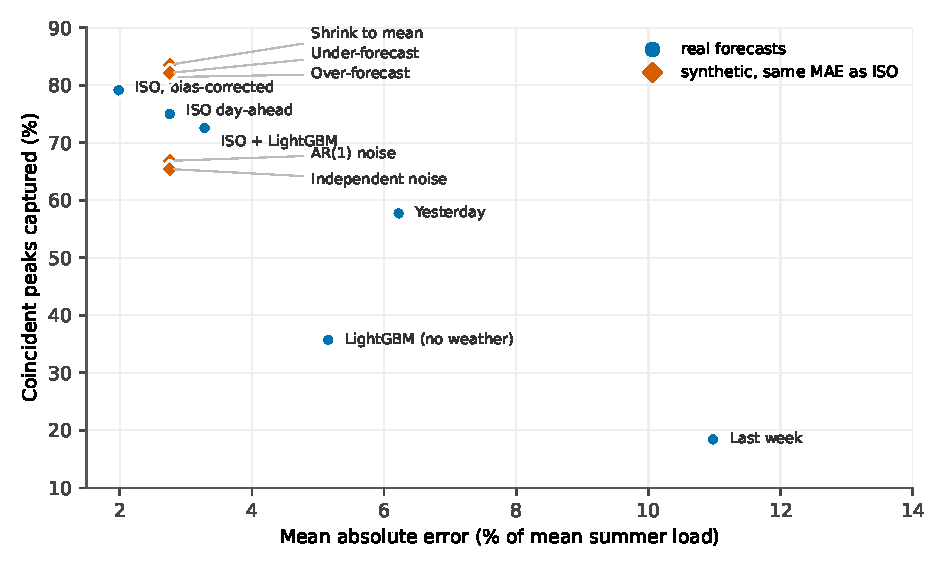
\includegraphics[width=0.92\linewidth]{fig_capture_mae.pdf}
\caption{Share of coincident-peak hours captured against the mean absolute error, primary policy, averaged over \res{nMarketYears} market-years. Synthetic forecasts (diamonds) all have the same error as the ISO forecast in each market-year.}
\label{fig:cap}
\end{figure}

\begin{table}[t]
\centering
\caption{Share of coincident-peak hours captured (\%) by market, primary policy (three-hour window, budget five times the number of CPs).}
\label{tab:market}
\small
\setlength{\tabcolsep}{4pt}
\begin{tabular}{lrrrrrrrr}
\toprule
Market & CPs & Budget & ISO & ISO bc & LightGBM & Yesterday & Shrink & Noise \\
\midrule
ERCOT 4CP & \res{nCPErcot} & \res{budgetErcot} & \res{capIsoErcot} & \res{capIsobcErcot} & \res{capMlErcot} & \res{capPersErcot} & \res{capShrinkErcot} & \res{capNoiseErcot} \\
PJM 5CP & \res{nCPPjm} & \res{budgetPjm} & \res{capIsoPjm} & \res{capIsobcPjm} & \res{capMlPjm} & \res{capPersPjm} & \res{capShrinkPjm} & \res{capNoisePjm} \\
NYISO & \res{nCPNyiso} & \res{budgetNyiso} & \res{capIsoNyiso} & \res{capIsobcNyiso} & \res{capMlNyiso} & \res{capPersNyiso} & \res{capShrinkNyiso} & \res{capNoiseNyiso} \\
ISO-NE & \res{nCPIsone} & \res{budgetIsone} & \res{capIsoIsone} & \res{capIsobcIsone} & \res{capMlIsone} & \res{capPersIsone} & \res{capShrinkIsone} & \res{capNoiseIsone} \\
\bottomrule
\end{tabular}
\end{table}

\subsection{The form of the error}

The five synthetic forecasts share the ISO forecast's error in every market-year, yet their capture spanned \res{synSpread} percentage points (Figure~\ref{fig:types}). Forecasts whose error keeps the order of days did best: a constant over-forecast caught \res{capBias}\% of CPs, a constant under-forecast \res{capUnder}\%, and shrink to mean \res{capShrink}\%. Noise did worst: \res{capArone}\% with autocorrelated and \res{capNoise}\% with independent noise.

\emph{H2 was not supported, and the data point the other way.} Shrink to mean captured more CPs, not fewer, than over-forecast, under-forecast and noise (one-sided $p=\res{hTwoPBias}$, \res{hTwoPUnder} and \res{hTwoPNoise}). Pulling every hour towards its recent mean compresses the peaks but almost preserves their order, and the primary policy, which sets thresholds on the forecast's own scale, recalibrates to the compressed scale. In the exactly-$B$ policy, which depends only on order, a constant bias caught \res{capBiasExact}\% and shrink to mean \res{capShrinkExact}\% of CPs, against \res{capNoiseExact}\% for independent noise.

How the forecast is used decides whether compression is harmless. When the threshold and running maximum came from actual past peaks, shrink to mean caught only \res{capShrinkActual}\% of CPs, because its compressed peaks rarely reached the actual-scale threshold, while a constant over-forecast caught \res{capBiasActual}\%.

\begin{figure}[t]
\centering
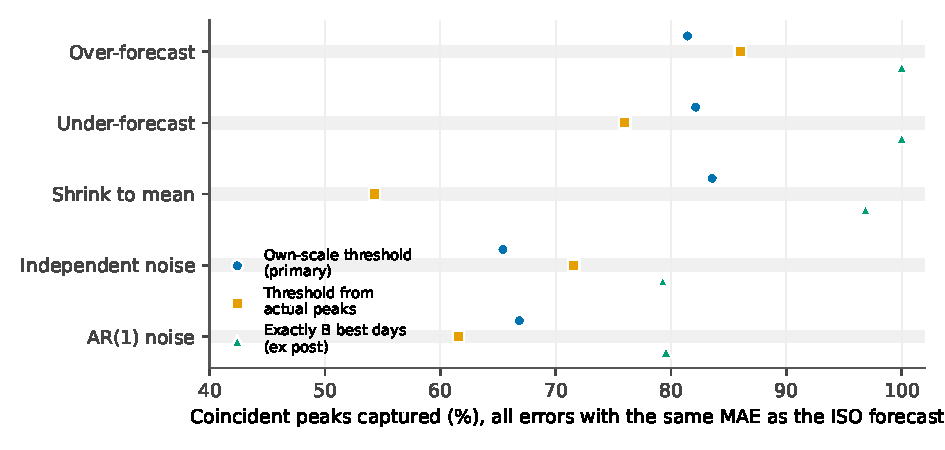
\includegraphics[width=0.95\linewidth]{fig_error_types.pdf}
\caption{Coincident peaks captured by five synthetic forecasts with the same mean absolute error as the ISO forecast, under three ways of using the forecast: thresholds on the forecast's own scale (primary), thresholds from actual past peaks, and the ex post choice of the $B$ days with the highest forecast peaks.}
\label{fig:types}
\end{figure}

\subsection{Ranking the top days}

\emph{H3 was supported.} The tail-rank score was more strongly associated with capture than MAE: mean Kendall $\tau=\res{hThreeTail}$ against $\res{hOneTau}$ (paired bootstrap, one-sided $p\res{hThreeP}$). Within the synthetic group, where MAE is constant by construction, the tail-rank score still ordered capture ($\tau=\res{tauSynTail}$, exploratory). On average the ISO forecast's tail-rank score was \res{tailIso}, that of the bias-corrected ISO forecast \res{tailIsobc} and that of LightGBM \res{tailMl}.

\subsection{Operator forecasts and a weather-free model}

\emph{H4 was supported.} The ISO forecast captured at least as many CPs as LightGBM in every market and more in all four: ERCOT \res{hFourIsoErcot} against \res{hFourMlErcot} of \res{hFourNErcot}, PJM \res{hFourIsoPjm} against \res{hFourMlPjm} of \res{hFourNPjm}, NYISO \res{hFourIsoNyiso} against \res{hFourMlNyiso} of \res{hFourNNyiso}, and ISO-NE \res{hFourIsoIsone} against \res{hFourMlIsone} of \res{hFourNIsone}. LightGBM had no weather input, and a weather-driven model would likely do better; the comparison shows that the operators' forecasts, which include weather, are a strong free baseline.

\subsection{Robustness}

Table~\ref{tab:robust} reports the two correlations and the capture of the five synthetic forecasts under the secondary configurations. Across all \res{nConfigs} combinations of policy, budget and window, the mean correlation between MAE and capture ranged from \res{tauAllMin} to \res{tauAllMax} and that between the tail-rank score and capture from \res{tailAllMin} to \res{tailAllMax}; the tail-rank score had the larger correlation in every combination, although the difference was not statistically significant in all of them. Excluding 2020 changed neither ($\tau=\res{tauNoCovid}$ and \res{tailNoCovid}). Capture was much lower in ERCOT and PJM, with four or five CPs a year to find, than in NYISO and ISO-NE, with one (Table~\ref{tab:market}).

\begin{table}[t]
\centering
\caption{Robustness. Mean within-market-year Kendall $\tau$ of capture with MAE and with the tail-rank score, and the capture (\%) of the same-MAE synthetic forecasts, under the primary and secondary configurations (budget multiple of the number of CPs; window in hours).}
\label{tab:robust}
\small
\setlength{\tabcolsep}{4pt}
\begin{tabular}{lrrrrrrr}
\toprule
Configuration & $\tau$ MAE & $\tau$ tail & Over & Under & Shrink & Noise & AR(1) \\
\midrule
Primary (own scale, $\times5$, 3 h) & \res{hOneTau} & \res{hThreeTail} & \res{capBias} & \res{capUnder} & \res{capShrink} & \res{capNoise} & \res{capArone} \\
Threshold from actual peaks & \res{tauActual} & \res{tailActual} & \res{capBiasActual} & \res{capUnderActual} & \res{capShrinkActual} & \res{capNoiseActual} & \res{capAroneActual} \\
Exactly $B$ days (ex post) & \res{tauExact} & \res{tailExact} & \res{capBiasExact} & \res{capUnderExact} & \res{capShrinkExact} & \res{capNoiseExact} & \res{capAroneExact} \\
Budget $\times3$ & \res{tauMthree} & \res{tailMthree} & \res{capBiasMthree} & \res{capUnderMthree} & \res{capShrinkMthree} & \res{capNoiseMthree} & \res{capAroneMthree} \\
Budget $\times8$ & \res{tauMeight} & \res{tailMeight} & \res{capBiasMeight} & \res{capUnderMeight} & \res{capShrinkMeight} & \res{capNoiseMeight} & \res{capAroneMeight} \\
Window 1 h & \res{tauWone} & \res{tailWone} & \res{capBiasWone} & \res{capUnderWone} & \res{capShrinkWone} & \res{capNoiseWone} & \res{capAroneWone} \\
Window 5 h & \res{tauWfive} & \res{tailWfive} & \res{capBiasWfive} & \res{capUnderWfive} & \res{capShrinkWfive} & \res{capNoiseWfive} & \res{capAroneWfive} \\
\bottomrule
\end{tabular}
\end{table}

\section{Discussion}

Accuracy matters for catching coincident peaks: across forecasts that differ widely in quality, the more accurate ones caught more peaks, and correcting the operator forecast's recent bias both reduced its error and raised its capture. Accuracy and decision value can come apart in other problems \citep{murphy1993good,elmachtoub2022spo}; here they move together, because a CP alert is a ranking decision: what the customer needs is the order of the season's top days, and large errors of the kind that yesterday's or last week's load make also scramble that order.

Accuracy is not the whole story, however. Errors of the same size differed by up to \res{synSpread} percentage points in capture, depending on whether they preserved the order of days. A constant bias, which inflates the MAE, is nearly harmless for a policy that sets its thresholds on the forecast's own history, and so is the shrinkage towards the mean that statistical models produce at extremes. Both become harmful when a customer compares the forecast with actual past peaks, a natural thing to do with a vendor's numbers: a compressed forecast then seldom crosses the actual-scale threshold. The same forecast can thus be valuable or poor depending on how it is used.

Three practical recommendations follow. Customers and vendors should evaluate CP forecasts by how they rank the top days of each period, for example with the tail-rank score used here, rather than by the MAE over all hours. Alert thresholds should be calibrated on the forecast's own past values, not on actual peaks, unless the forecast is known to be unbiased at the extremes. And the operators' free day-ahead forecasts, especially after a simple 28-day bias correction, are a hard baseline that any paid service should be required to beat on capture, not on accuracy.

\subsection{Limitations}

CP hours were identified from hourly data; ERCOT uses 15-minute intervals, so a small number of official CP intervals may fall in a different hour. The policies are stylised: real customers use intraday updates, weather forecasts and judgement, and the CP itself can move when many customers curtail at once \citep{zhang2026cp}, which this study cannot capture with realised loads. The machine-learning model was deliberately simple and weather-free. Synthetic forecasts were matched to the ISO forecast's error per market-year; other error magnitudes were not explored. The study covers nine summers in four markets; with one CP a year in NYISO and ISO-NE, per-market comparisons there rest on nine peaks. The analysis plan was amended three times (Section~\ref{sec:plan}), once after the full run to remove recording errors; the unscreened results, reported, led to the same conclusions.

\section{Conclusions}

A more accurate day-ahead load forecast does catch more coincident peaks, but the form of its error matters as much as its size: errors that keep the order of days caught \res{capBias}--\res{capShrink}\% of the peaks, and noisy errors of the same size only \res{capNoise}--\res{capArone}\%. Forecasts for coincident-peak management should be judged by how well they rank the season's top days and used with thresholds calibrated on their own scale.

\section*{Data availability}
EIA-930 data are public \citep{eia930}. The analysis plan with its commit history, the code, the download script with file hashes and the result files are available at \repolink.

\ifdefined\ANON\else
\section*{CRediT authorship contribution statement}
\textbf{Thanh Van Nguyen:} Conceptualization, Methodology, Software, Formal analysis, Data curation, Writing -- original draft, Writing -- review \& editing.
\fi

\section*{Declaration of generative AI and AI-assisted technologies in the writing process}
During the preparation of this work the author used Claude Opus 5.5 (Anthropic; used in November 2026 through Claude Code) to help design the analysis, write and test the code, search the literature and check every reference against Crossref and arXiv, obtain a referee-style critique of the draft, and draft and edit the text. The author chose the research question, approved the analysis plan and each amendment, and checked the results. After using this tool, the author reviewed and edited the content as needed and takes full responsibility for the content of the published article.

\section*{Declaration of competing interest}
The author declares no known competing financial interests or personal relationships that could have appeared to influence the work reported in this paper.

\section*{Funding}
This research did not receive any specific grant from funding agencies in the public, commercial, or not-for-profit sectors.

\bibliographystyle{unsrtnat}
\bibliography{refs}

\end{document}
